\begin{figure}[H]
    \centering
    \begin{subfigure}{.3\textwidth}
        \centering
        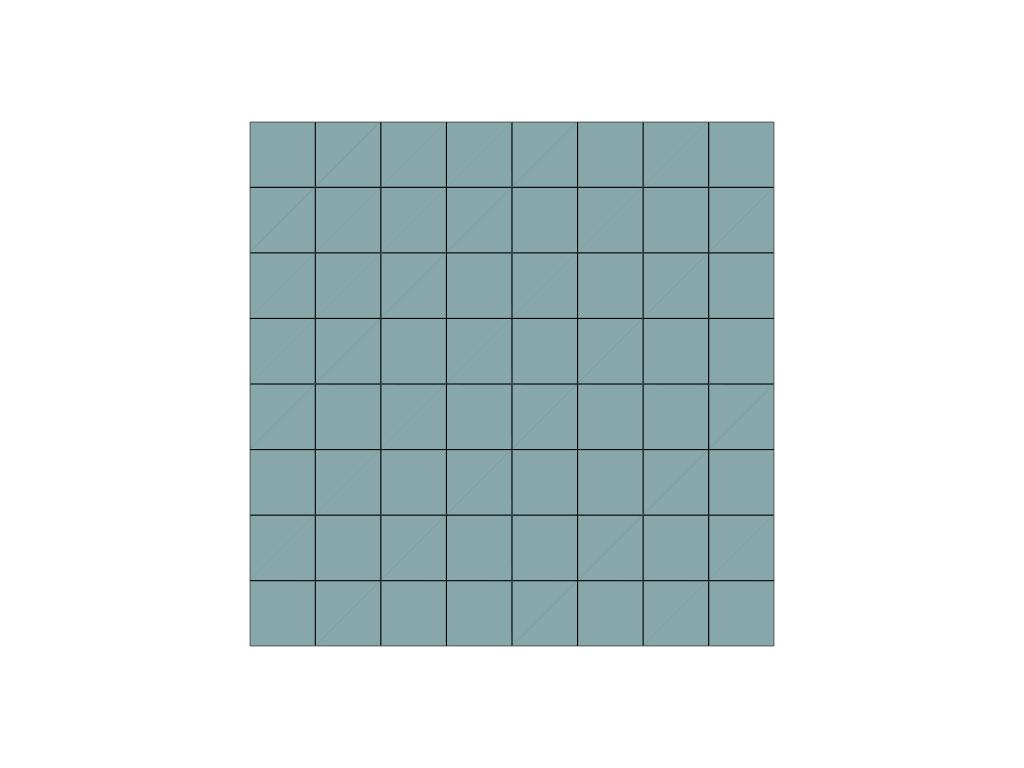
\includegraphics[width=\textwidth]{Afsnit/Application/figurer/screenshot_1.jpeg}
        \caption{Quadrilaterial slicing of domain}~\label{fig:FEM_plot_domain}
      \end{subfigure}
    \begin{subfigure}{.3\textwidth}
        \centering
        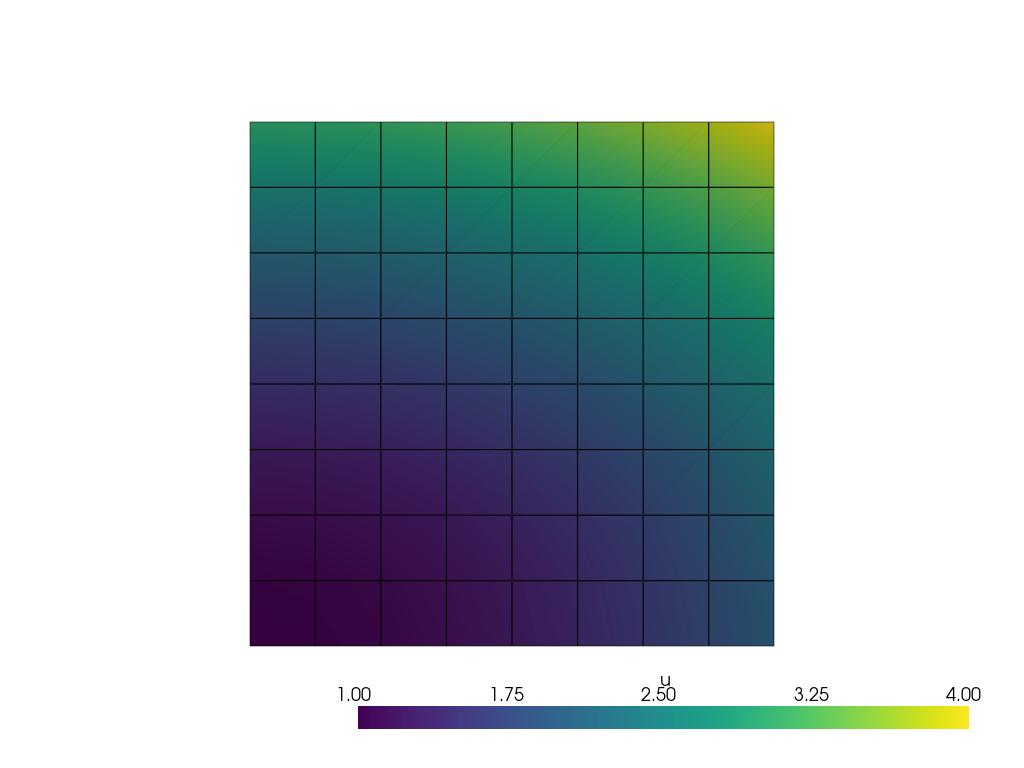
\includegraphics[width=\textwidth]{Afsnit/Application/figurer/screenshot_2.jpeg}
        \caption{Domain colored in accordance to the warping scalar obtained by the solution $u_h$ ranging from 1 to 4}~\label{fig:FEM_plot_warped_domain}
    \end{subfigure}
    \begin{subfigure}{.3\textwidth}
        \centering
        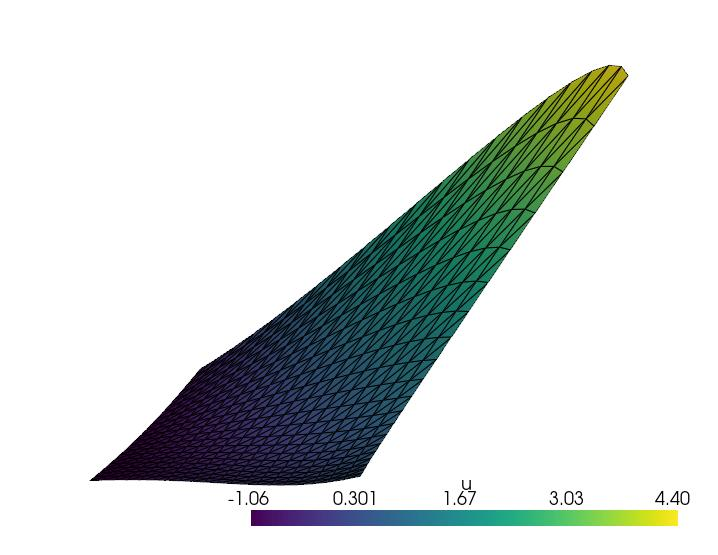
\includegraphics[width=\textwidth]{Afsnit/Application/figurer/screenshot_3.jpeg}
        \caption{The same domain warped with respect to the scalar value, ranging from 1 to 4}~\label{fig:FEM_plot_3D}
    \end{subfigure}
    \caption{Plots of the ?quadrilaterialerised? domain}~\label{fig:FEM_plots}
\end{figure}

As discussed earlier the first step in approximatin the solution to a partial differential equation is do establish a fitting domain. In our example we have chosen a square ranging from $(-1,-1)$ to $(1,1)$.
The domain is then quadrilaterialerised or triangulised depending on the specific scenario, in Plot~\ref{fig:FEM_plot_domain} we have chosen to slice the domain into quadrilaterials, of equal size making the domain regular.
After the domain is sliced and we have estimated the soltion using the nodal points obtained in the quadrilaterials, we can plot the solution over the domain to obtain Plot~\refeq{fig:FEM_plot_warped_domain} where each cell is colored in accordance to the value in the given point.
We can then warp the domain to give a clear look on what exactly our solution looks like in 3D, this is shown in Plot~\refeq{fig:FEM_plot_3D}, where it is also obvious what the visual meaning of a boundary condition, since it is clear the boundary follows the specificied function $1 + x_0^2 + 2x_1^2$.